\documentclass{beamer}


\usetheme{default}
\usepackage{subfigure}
\usepackage{amsmath}
\usepackage{Sweave}
\usepackage{graphicx}
\usepackage{color}
\usepackage{amsfonts}
\usepackage{amssymb}
\usepackage{multicol}
\usepackage[all]{xy}
\usepackage{bm}


\author{Patrick Lam}
\title{Maximum Likelihood}
\date{}
%\date{February 26, 2009}

\begin{document}

\newcommand{\red}{\textcolor{red}}
\newcommand{\blue}{\textcolor{blue}}
\newcommand{\purple}{\textcolor{purple}}
\newcommand{\brown}{\textcolor{brown}}

\frame{\titlepage}

\begin{frame}
\frametitle{Maximum Likelihood}
\pause
Suppose we have some data $y$ and we want to find some parameters
$\theta$ that generated $y$.\\
\pause
\bigskip
Maximum likelihood is a way to find $\theta$.
\end{frame}

\begin{frame}
\frametitle{Derived from Bayes' Rule}
\pause
Assume that $y$ follows some distribution $p(y | \theta)$.
\pause
\begin{eqnarray*}
\blue{p(\theta | y)} &=& \frac{p(y | \theta) \red{p(\theta)}}{\brown{p(y)}}\\
\pause
\blue{p(\theta | y)} &=& p(y | \theta) \purple{k(y)} \\
\pause
\blue{p(\theta | y)} &\propto& p(y | \theta) \\\\
\pause
L(\theta | y) &=& p(y|\theta)
\end{eqnarray*}
\pause
The likelihood function is mathematically the same as the distribution
for $y$. \\
\pause 
\bigskip 
Our best estimate of $\theta$ (MLE) is the value of $\theta$
that maximizes the likelihood function. \pause Why? \pause and why? 
\end{frame}

\begin{frame}
\frametitle{Why Does $L(\theta | y) = p(y | \theta)$ work?}
\pause
Suppose we have one observation $y = 0.5$ (assumed to be) drawn from a
Normal distribution with $\sigma^2 = 1$. \\
\bigskip
\pause
Estimate the mean $\mu$ of the distribution. \\
\bigskip
\pause
Obvious guess: $\mu = 0.5$

\end{frame}

\begin{frame}
\begin{figure}
\subfigure{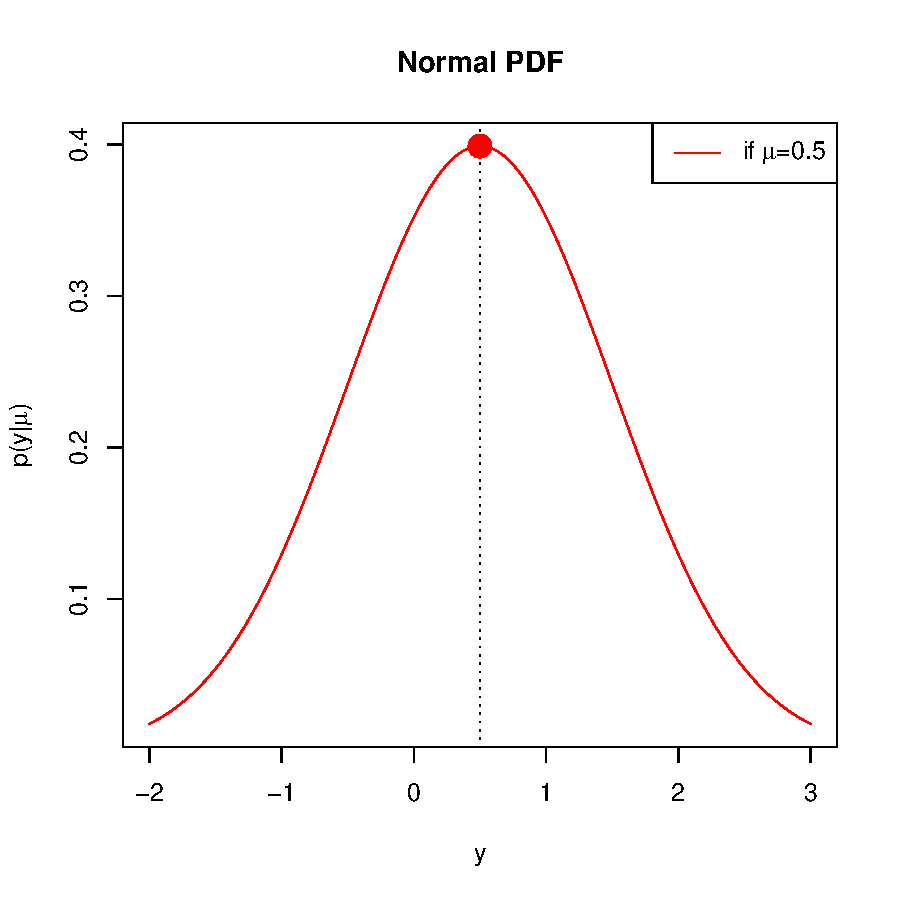
\includegraphics[width=2in, height=2in]{maxlik-lik1.pdf}}
\pause
\subfigure{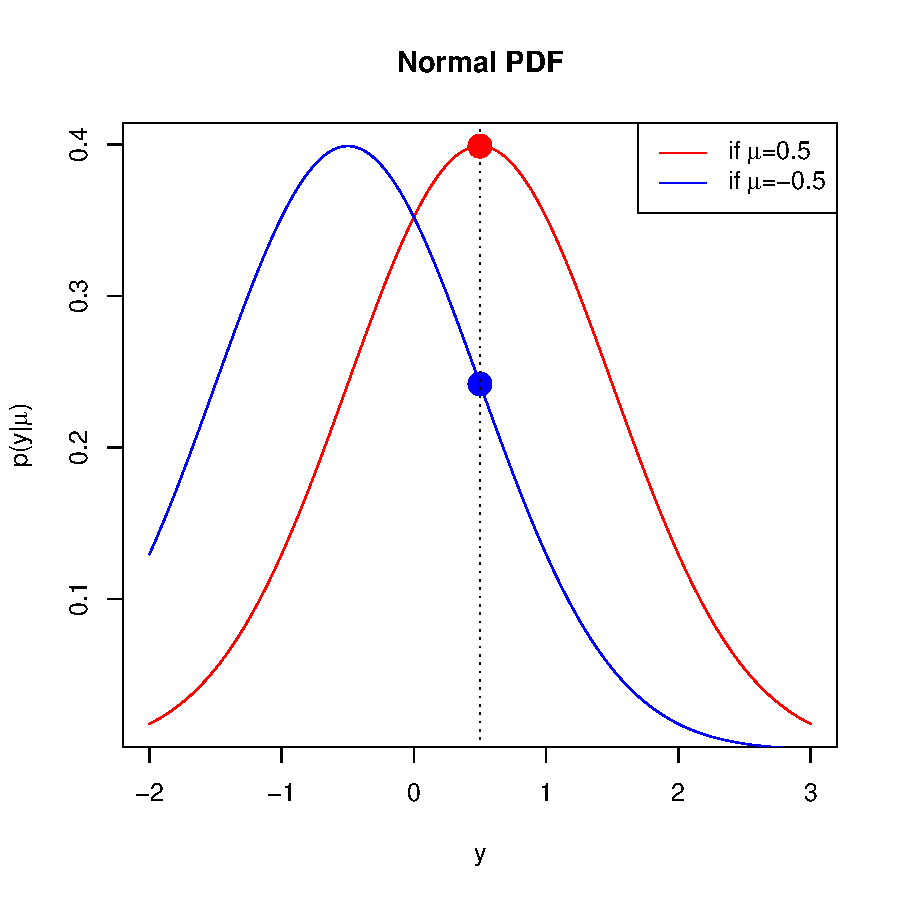
\includegraphics[width=2in, height=2in]{maxlik-lik2.pdf}}
\end{figure}
\end{frame}

\begin{frame}


\begin{figure}
\subfigure{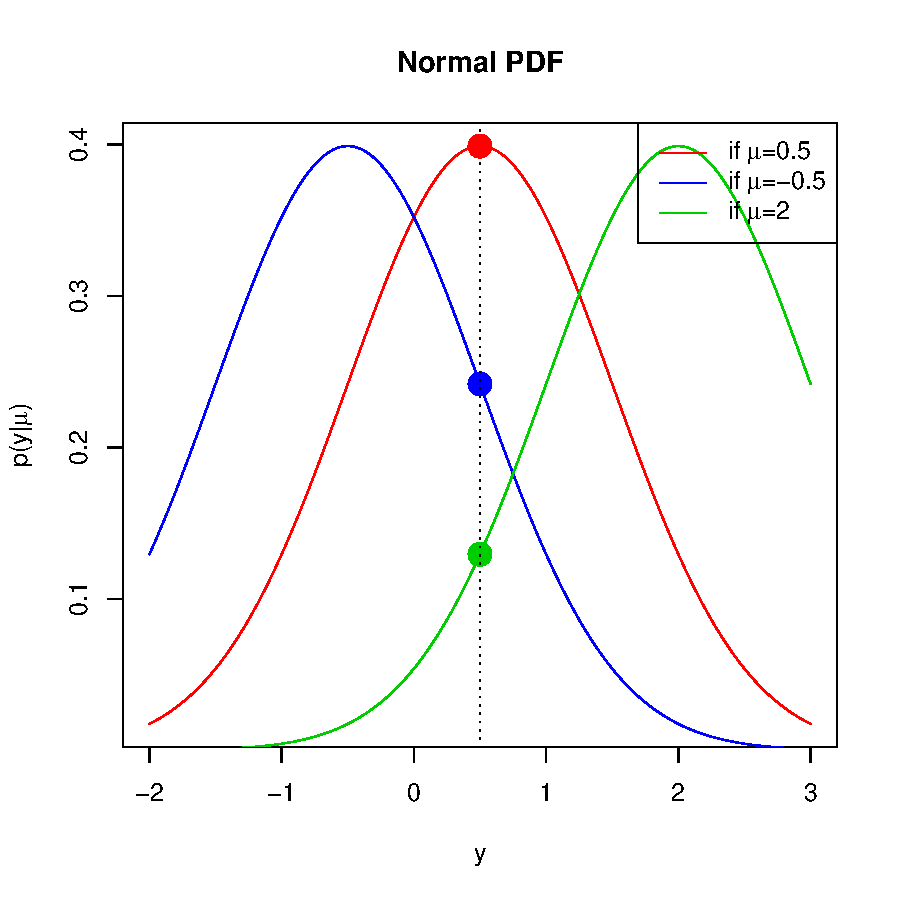
\includegraphics[width=2in, height=2in]{maxlik-lik3.pdf}}
\pause
\subfigure{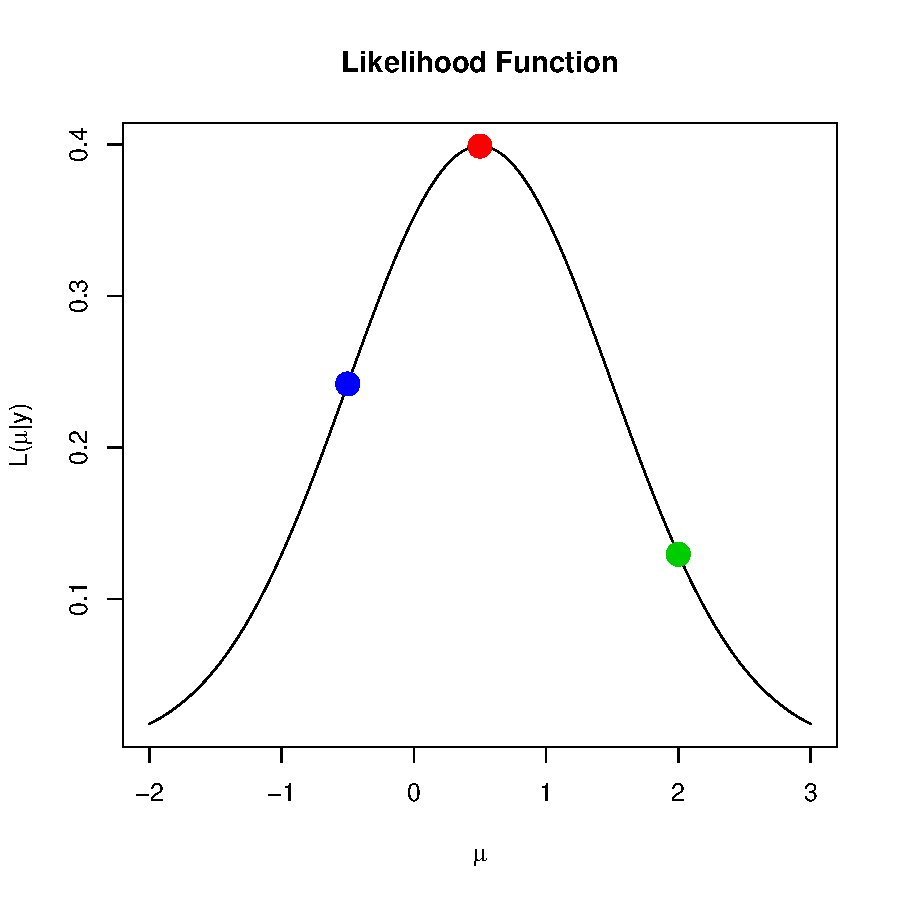
\includegraphics[width=2in, height=2in]{maxlik-lik4.pdf}}
\end{figure}

\pause
Our best estimate of $\theta$ is the value of $\theta$ that maximizes
$L(\theta | y)$ (MLE).
\end{frame}

\begin{frame}
\frametitle{Example: Poisson Distribution}
Suppose we have some count data (number of coups in a year). \\
\pause 
\bigskip
We can use a Poisson distribution to model the data (we will learn more about
Poisson later).
\pause
\begin{eqnarray*}
Y_i \sim_{iid} \mathrm{Poisson}(\lambda)
\end{eqnarray*}
\pause
We want to find $\lambda$, which is the mean of the Poisson
distribution.\\ \pause 
\bigskip
The PMF (discrete) for the data is
\begin{eqnarray*}
p(\mathbf{y} | \lambda) &=& \prod_{i=1}^n \frac{\lambda^{y_i} e^{-\lambda}}{y_i!}
\end{eqnarray*}
\end{frame}

\begin{frame}
Since $L(\theta | y) = p(y | \theta)$, we have
\begin{eqnarray*}
L(\lambda | \mathbf{y}) &=& \prod_{i=1}^n \frac{\lambda^{y_i} e^{-\lambda}}{y_i!}
\end{eqnarray*}
\pause
To make the math easier, we will take the log-likelihood.
\pause
\begin{eqnarray*}
l(\lambda | \mathbf{y}) &=& \sum_{i=1}^n \left( y_i \, \mathrm{ln} \, \lambda
- \lambda - \red{\mathrm{ln} \, y_i!} \right)
\end{eqnarray*}
\pause
We can drop all terms that don't depend on $\lambda$ (because
likelihood is a relative concept and is invariant to shifts).
\pause
\begin{eqnarray*}
l(\lambda | \mathbf{y}) &=& \sum_{i=1}^n (y_i \, \mathrm{ln} \, \lambda)
- n\lambda 
\end{eqnarray*}
\end{frame}

\begin{frame}
\frametitle{Why Can We Use the Log-likelihood?}
\pause


\begin{figure}
\begin{center}
\subfigure{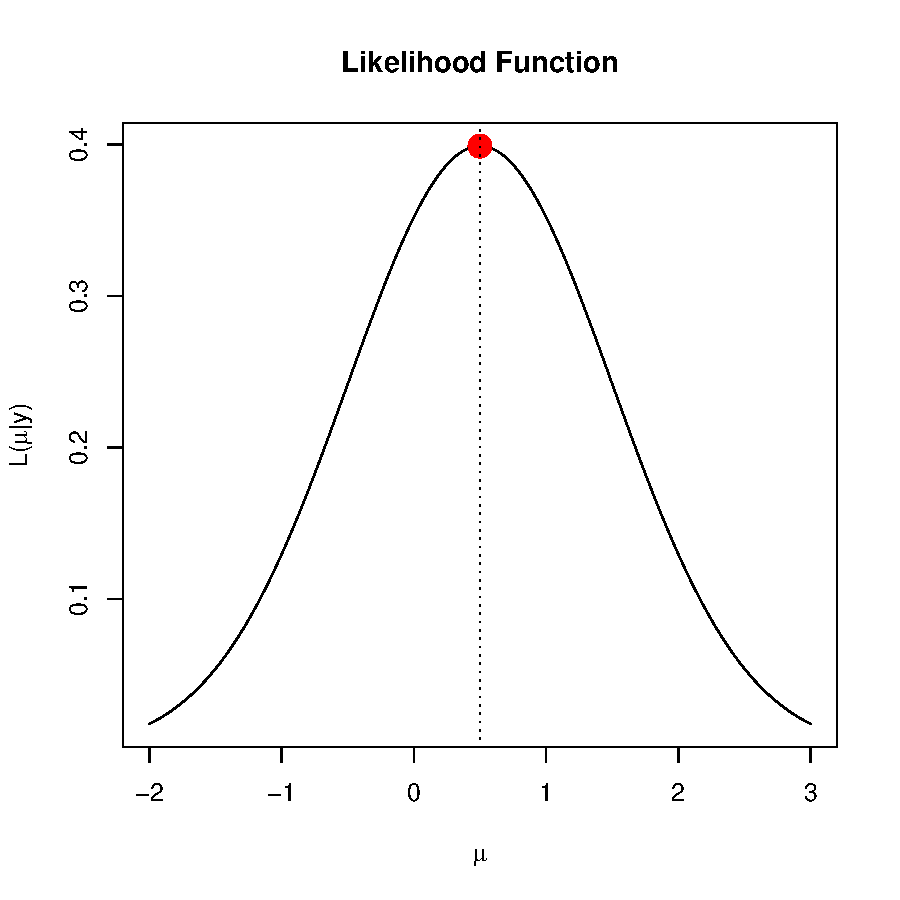
\includegraphics[width=2in, height=2in]{maxlik-loglik.pdf}}
\subfigure{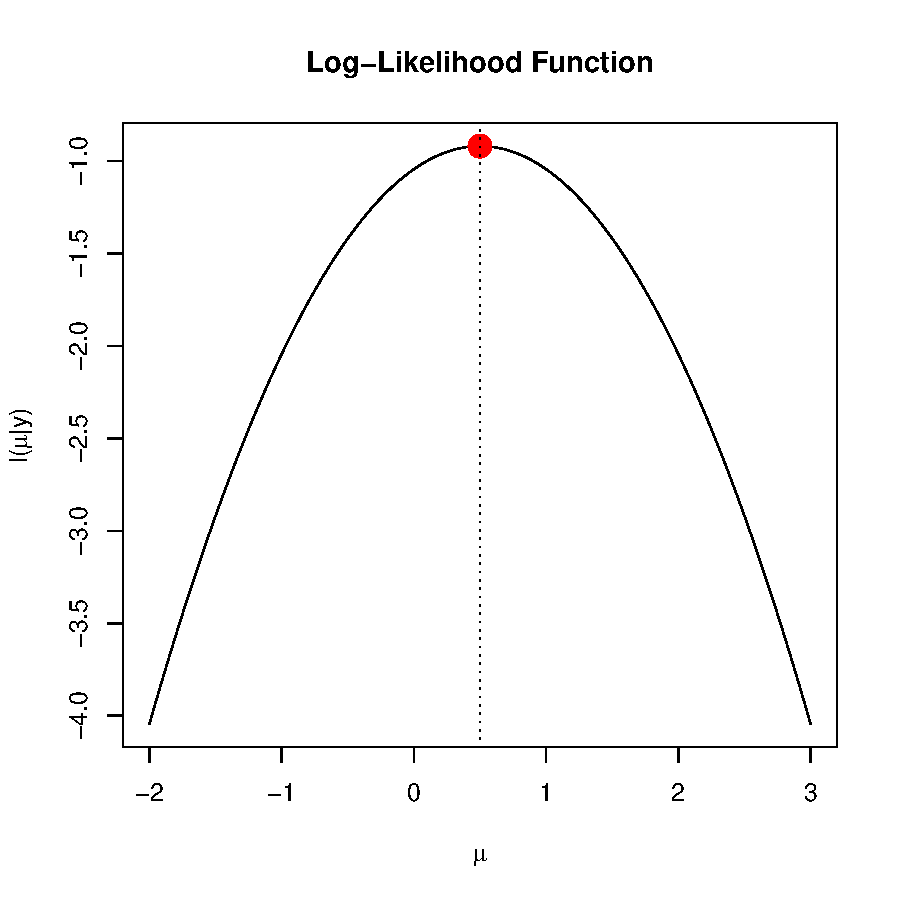
\includegraphics[width=2in, height=2in]{maxlik-loglik2.pdf}}
\end{center}
\end{figure}
\end{frame}

\begin{frame}
\frametitle{Finding the Maximum Likelihood Estimate (MLE)}
\pause
Remember that to find our MLE, we want to find the value of the
parameter(s) that maximizes our log-likelihood.
\pause
\begin{eqnarray*}
l(\lambda | \mathbf{y}) &=& \sum_{i=1}^n (y_i \, \mathrm{ln} \, \lambda)
- n\lambda 
\end{eqnarray*}
\pause
We need to set the derivative (known as the score function) to zero and solve for $\lambda$.
\pause
\begin{eqnarray*}
\frac{\partial l(\lambda | \mathbf{y}) }{\partial \lambda} = S(\theta)
&=& \frac{\sum_{i=1}^n y_i}{\lambda} - n \\
\pause
0 &=& \frac{\sum_{i=1}^n y_i}{\lambda} - n \\
\pause
\hat{\lambda} &=& \frac{\sum_{i=1}^n y_i}{n}
\end{eqnarray*}
\end{frame}

\begin{frame}[fragile]
\frametitle{Maximum Likelihood In R}
\pause
Write our log-likelihood function:
\pause
\begin{eqnarray*}
l(\lambda | \mathbf{y}) &=& \sum_{i=1}^n (y_i \, \mathrm{ln} \, \lambda)
- n\lambda 
\end{eqnarray*}
\pause
\tiny
\begin{Schunk}
\begin{Sinput}
> ll.poisson <- function(par, y) {
+     lambda <- exp(par)
+     out <- sum(y * log(lambda)) - length(y) * lambda
+     return(out)
+ }
\end{Sinput}
\end{Schunk}
\pause
\normalsize
\bigskip
Find the maximum (with sample data) 
\tiny
\begin{Schunk}
\begin{Sinput}
> y <- rpois(1000, 5)
> opt <- optim(par = 2, fn = ll.poisson, method = "BFGS", control = list(fnscale = -1), 
+     y = y)$par
> mle <- exp(opt)
> mle
\end{Sinput}
\begin{Soutput}
[1] 4.996001
\end{Soutput}
\end{Schunk}
\normalsize
\pause
What the exp()?
\end{frame}

\begin{frame}
\frametitle{Reparameterization}
\pause
We need to reparameterize the parameters in our function to constrain
the search space. \\
\pause
\bigskip
We also need to reparameterize the output from {\tt optim()}. \\
\bigskip
\pause
Likelihood is invariant to reparameterization. \\
\bigskip
\pause
Common reparameterizations:
\pause
\begin{itemize}
\item To constrain to positive space: \pause {\tt exp()}
\pause
\item To constrain to $[0,1]$, \pause use a cdf
\end{itemize}
\end{frame}

\begin{frame}
\frametitle{Cumulative Distribution Function}
\pause
We've learned how to define a distribution via is PDF or PMF f(x). \\
\pause
\bigskip
Every distribution also has a CDF F(x): \pause $P(X \le x)$\\
\pause
\bigskip
For discrete case:
\begin{eqnarray*}
F(x) = P(X \le x) = \sum_{x_i \le x} P(X = x_i)
\end{eqnarray*}
\pause
For continuous case:
\begin{eqnarray*}
F(x) = \int_{-\infty}^x f(t) dt
\end{eqnarray*}
\end{frame}

\begin{frame}
\frametitle{Standard Normal PDF and CDF}
\begin{figure}
\begin{center}
\subfigure{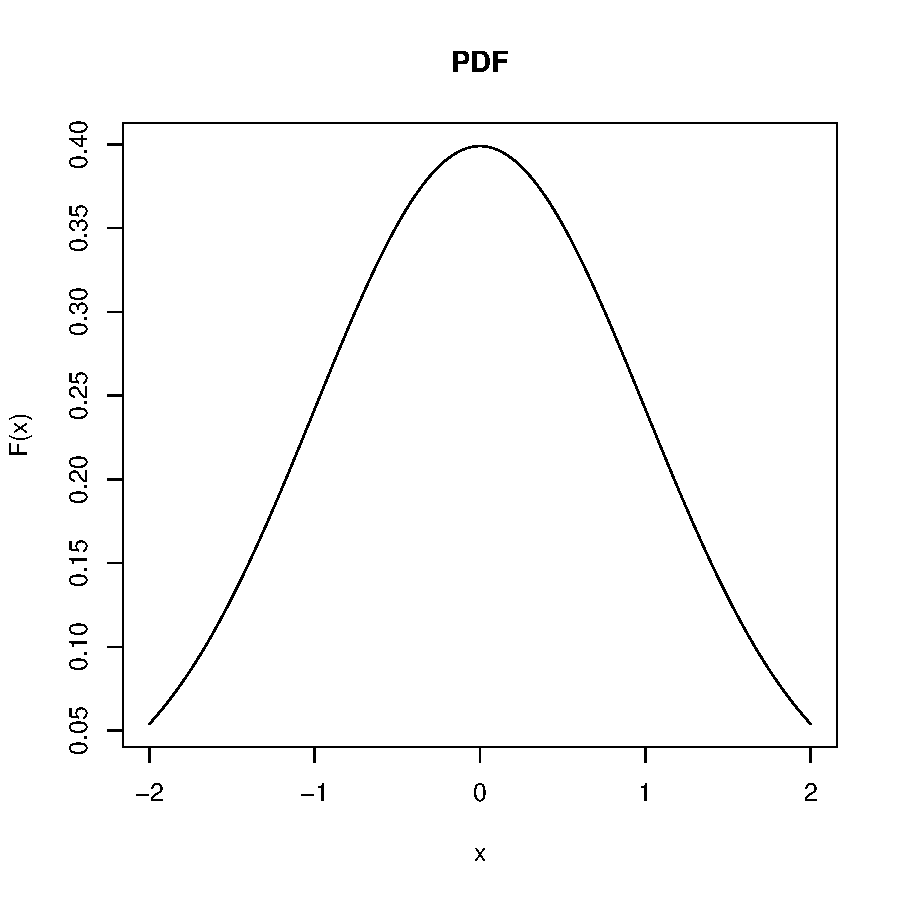
\includegraphics[width=2in, height=2in]{maxlik-normalpdf.pdf}}
\subfigure{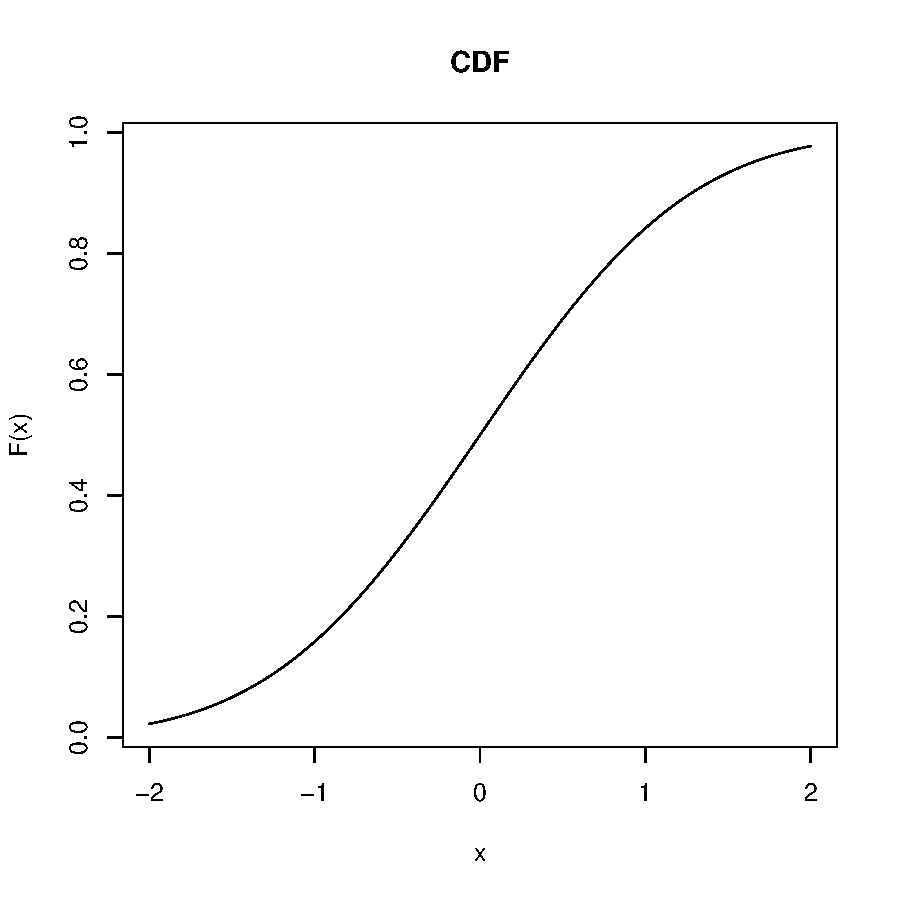
\includegraphics[width=2in, height=2in]{maxlik-normalcdf.pdf}}
\end{center}
\end{figure}
\end{frame}

\begin{frame}
\frametitle{Poisson(5) PMF and CDF}
\begin{figure}
\begin{center}
\subfigure{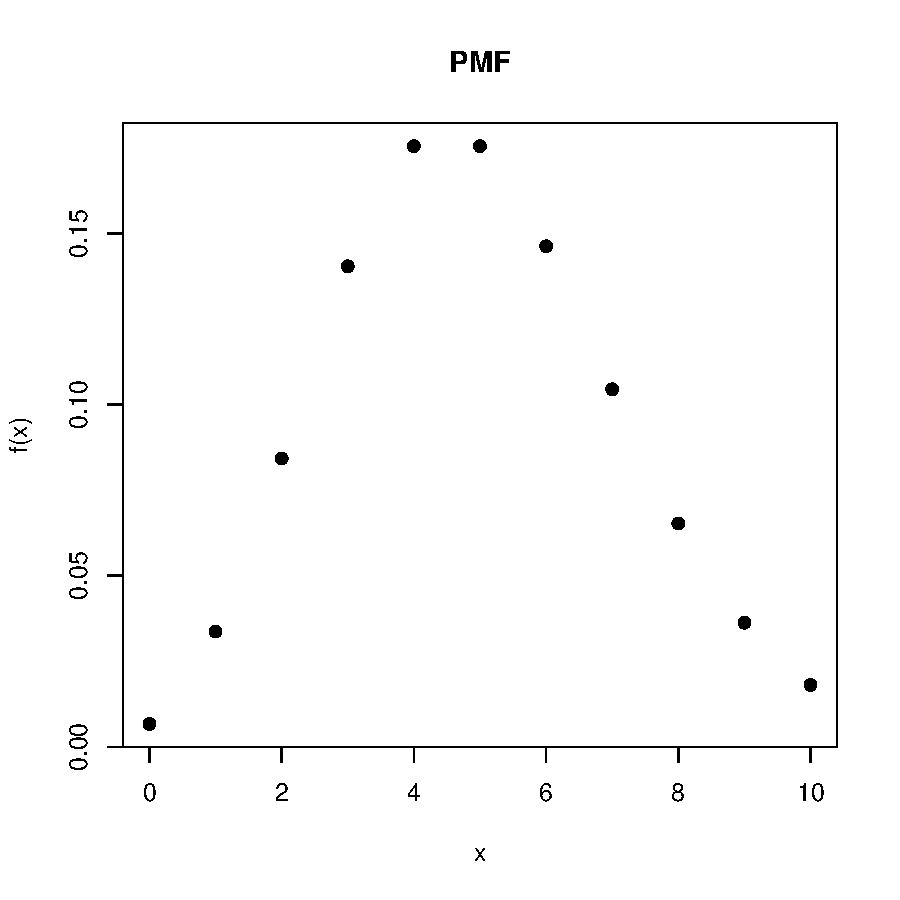
\includegraphics[width=2in, height=2in]{maxlik-poispdf.pdf}}
\subfigure{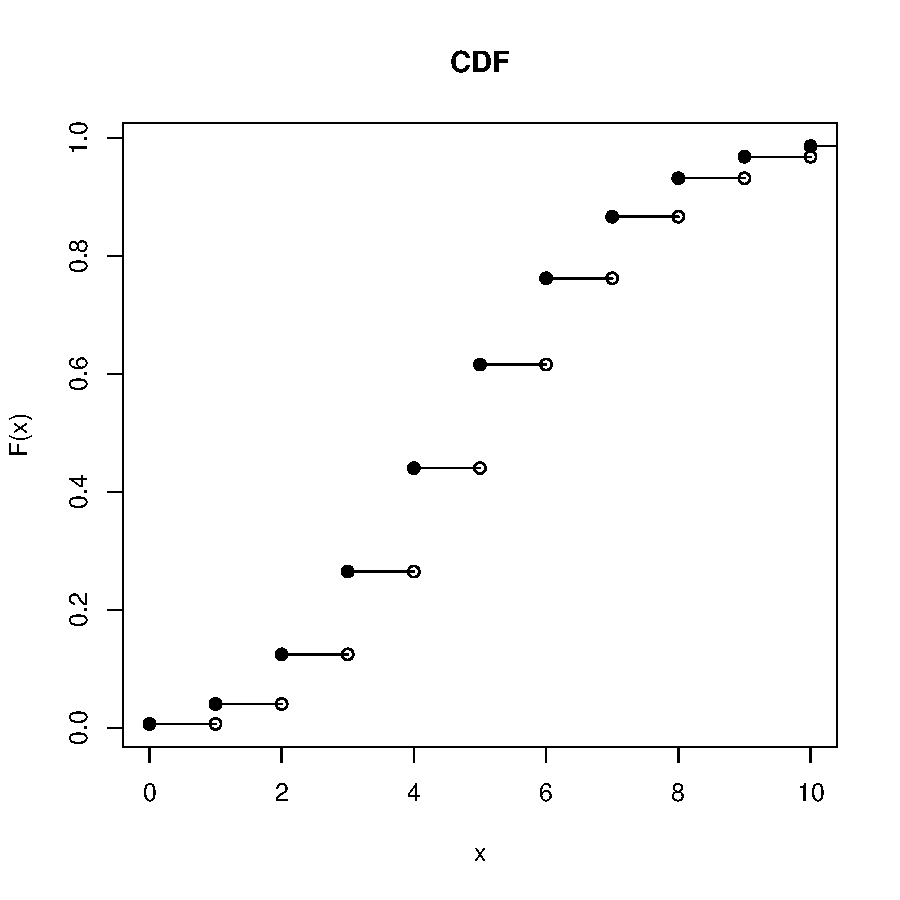
\includegraphics[width=2in, height=2in]{maxlik-poiscdf.pdf}}
\end{center}
\end{figure}
\end{frame}

\begin{frame}
We can use a CDF to transform numbers from $(-\infty, \infty)$ to $[0,1]$.\\
\bigskip
\pause
Commonly used: 
\pause
\begin{itemize}
\item Standard Normal CDF: $\Phi(\cdot)$\\
\pause
\item Logistic CDF: $\frac{1}{1 + e^{-x}}$
\end{itemize}
\pause
\bigskip
\bigskip
Why shouldn't we use a CDF of a discrete variable?\\
\pause
\bigskip
What about the CDF of a bounded variable?
\end{frame}

\begin{frame}
\frametitle{More Complicated Likelihoods}
\pause
Up to this point, our distributions have been relatively simple
(i.e. all observations are i.i.d. from a distribution with the same parameter).\\
\pause
\bigskip
Suppose our observations come from different distributions, or some
observations are not fully observed.  \\
\pause
\bigskip
How do we define the joint distribution for our data (and thus our likelihood)?\\
\pause
\bigskip
Use an indicator variable.
\end{frame}

\begin{frame}
\frametitle{Indicator Variable}
Let $D$ be an indicator variable such that $d_i = 1$ if $i$ follows
one distribution, and $d_i = 0$ if $i$ follows another distribution.\\
\pause
\bigskip
We can incorporate the indicator variable into our likelihood.
\end{frame}

\begin{frame}
\frametitle{Example 1}
\pause
Suppose that we have 5 observations.  The first 2 are assumed to be
from distribution 1.  The last 3 are assumed to be from distribution 2.
\pause
\bigskip
\begin{eqnarray*}
d &=& c(1,1,0,0,0)\\
\pause
p(\theta_1, \theta_2 | \mathbf{y}) &=& \prod_{i=1}^n [p(y_i |
\theta_1)]^{d_i} [p(y_i | \theta_2)]^{1-d_i}
\end{eqnarray*}
\end{frame}

\begin{frame}
\frametitle{Example 2}
\pause
Suppose that we have 5 observations.  We observe the first 2
observations completely, but we only observe that the last 3 are greater
than some number $z$. 
\pause
\bigskip
\begin{eqnarray*}
d &=& c(1,1,0,0,0)\\
\pause
p(\theta | \mathbf{y}) &=& \prod_{i=1}^n [p(y_i |
\theta)]^{d_i} [1 - F(z)]^{1-d_i}
\end{eqnarray*}
where $F(y)$ is the CDF for $p(y | \theta)$. \pause Remember
\begin{eqnarray*}
F(z) = P(Y \le z)
\end{eqnarray*}
\end{frame}

\end{document}
